\section{Pre-procesamiento}
\subsection{Introducción}
Cualquier problema en ciencia de datos, comienza con un estudio exhaustivo de los datos proporcionados y realizar un \textbf{procesamiento} previo.
Si este paso es omitido, los algoritmos no se comportarán de forma óptima, debido a  que van a lidiar con unos datos que tendrán valores perdidos, que no estén normalizados, datos des-balanceados, irrelevantes, entre otras problemas. El objetivo de esta fase, es realizar ciertas transformaciones sobres los datos en bruto filtrando esta información para que los algoritmos no tengan que enfrentarse a estos problemas.
\subsection{Análisis exploratorio de los datos}
Para comenzar, se empezó leyendo la documentación aportada con los datos, la cual contenía los siguientes campos:
\begin{itemize}
	\item \textbf{Nombre:} Nombre de la característica.
	\item \textbf{Descripción:} Breve resumen explicando el origen de la característica o el enunciado de la pregunta en la encuesta.
	\item \textbf{Valores:} Tipo y/o rango que toma la característica.
\end{itemize}

Esta información es muy útil, ya que aparte de darnos un poco más de conocimiento del objetivo que queremos alcanzar con estos datos, nos da información de algunas características redundantes.

\begin{table}[!htbp]
	\begin{tabular}{|l|l|l|}
		\cline{1-3}
		CF9  &	Normalmente es posible reducir...&	Respuesta: Verdadera/Falsa. \\ \cline{1-3}
		QF9	& Variable creada a partir de CF9.  & Valor 1 si la respuesta es correcta, 0 si no. \\ \cline{1-3}
	\end{tabular}
	\label{columnas_iguales}
	\caption{Comparación de dos características redundantes.}
\end{table}

Como podemos ver, estas dos columnas contienen información redundante, ya que siendo una respuesta de tipo verdadero o falso, tenemos dos columnas con la misma información. Este caso se repite en varios casos, y en todos ellos se ha optado por dejar unicamente la que tiene los valores numéricos.\\
\linebreak
El siguiente paso ha sido el de obtener las columnas que se van a usar como predictores.
La peculiaridad de este conjunto de datos tenemos 7 columnas que van a ser las que los algoritmos tienen que intentar predecir. De estas 7 columnas tenemos 6 de ellas que son de tipo ordinal, almacenando la opinión (en escala Likert) que ha tenido el entrevistado sobre la pregunta en concreto. La ultima de estas columnas es la media de las 6 columnas.\\
 A continuación se muestra una tabla con la ocurrencia de cada valor para las columnas que vamos a usar:\\
\linebreak
 \begin{figure}[!htbp]
 	 \centering
	 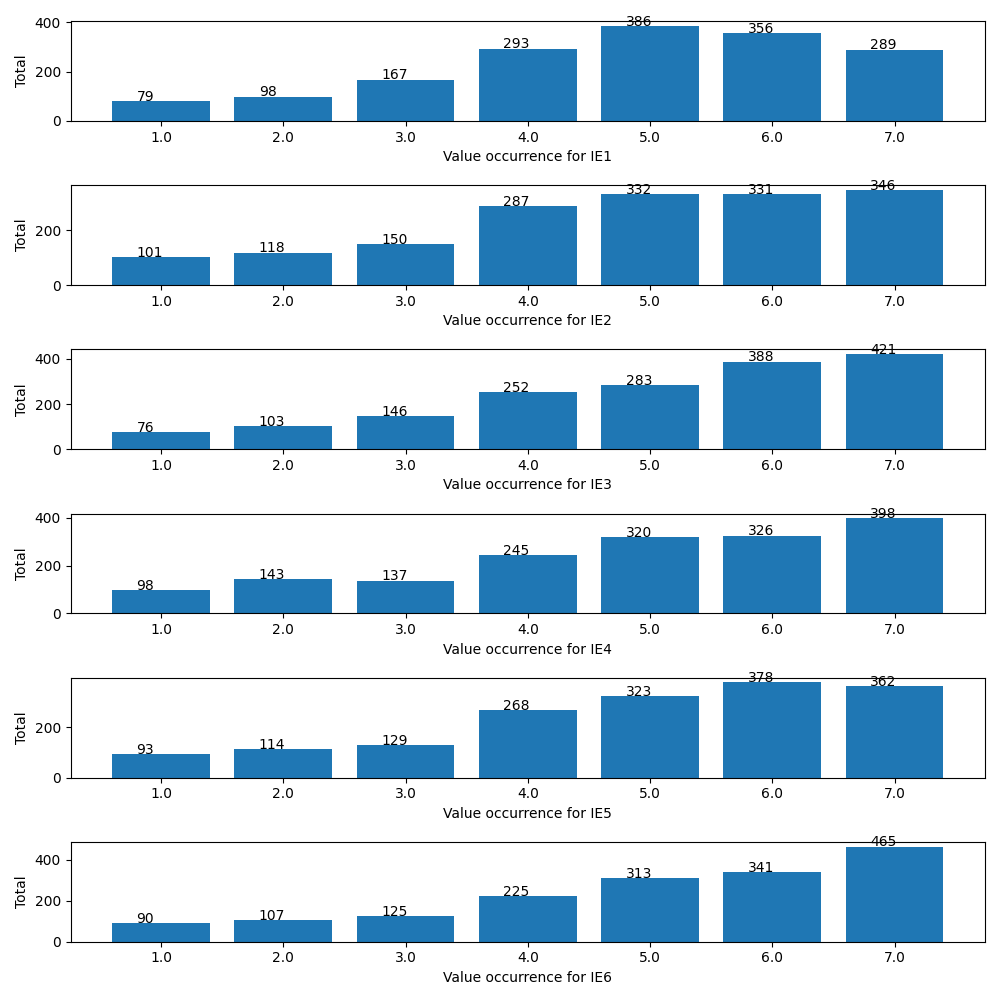
\includegraphics[scale=0.75]{value_occurrences.png}
	\caption{Conteo de valores para las columnas usadas como predictores}
	\label{ocurrencia_valores}
\end{figure}
\linebreak
Una vez leída esta documentación y detectados algunos casos de columnas con información redundante, se cargaron los datos y se sacaron una serie de métricas. Estamos ante un conjunto de datos formados por un total de 1672 ejemplos y con 246 características (antes de realizar cualquier tipo de procesamiento), las cuales pueden ser de tipo entero, flotante o categóricas.
\pagebreak
\subsection{Pre-procesado de datos}
En este paso también se han borrado aquellas columnas las cuales corresponden a respuestas de tipo abierta. Estas características pueden llegar a contener un valor único por cada uno de los ejemplos que tenemos. En un principio, van a ser descartadas, pero en fases siguientes se podría realizar un procesamiento más exhaustivo sobre dicha columna, agrupando ciertos valores y reduciendo así la complejidad. Cabe destacar que esta información no se esta perdiendo totalmente, ya que tenemos en todos los casos una nueva columna la cual contiene si la persona respondió correctamente o no a dicha pregunta. \\
\linebreak
Un caso particular que se detectó en esta fase, fue el de las características \textbf{BFx} y \textbf{BFxAdaptada} (hay un total de 4 columnas de este tipo). Las primeras columnas de este tipo, solo contenían la respuesta las personas que realizaron la entrevista en un único año, mientras que las columnas del segundo tipo contenían la respuestas de los dos años. Antes de eliminar las columnas del primer tipo, se realizo una comprobación para ver si realmente los datos comunes entre las dos columnas eran los mismos para así asegurar que no se están perdiendo datos.
\linebreak
El siguiente paso, ha sido analizar los valores únicos de cada variable, esto nos permitió detectar valores no validos. Se encontró los siguientes casos de valores nó validos:
\begin{itemize}
	\item \textbf{Valores perdidos especificados como espacios:} Si no procesamos estos valores, el algoritmo puede detectarlo como un valor válido, introduciendo así ruido en el modelo. Estos valores se cambiaron por \textit{NaN}.
	\item \textbf{Valores perdidos especificados como "\textit{No contesta}":} Estos valores se ven sobre todo en columnas con datos ordinales. El enfoque que se ha escogido ha sido el de cambiarlas por \textit{NaN}.
	\item \textbf{Valores inválidos en la columna "\textit{género}":} Según la documentación, los únicos valores que forman esta columna son \textit{hombre} y \textit{mujer}, pero dentro del conjunto de datos se detectan valores como \textit{si} y \textit{no}. No podemos saber si la persona que contestó la encuesta se equivocó ó le llegó una versión distinta de la encuesta, así que, estos valores dentro de la columna \textit{género} se reemplazaron por \textit{NaN}.
	\item \textbf{Valores binarios codificados como strings:} Este caso no es necesariamente un valor no válido, pero se decidió cambiar estos valores binarios codificados como \textit{sí} o \textit{no} por \textit{1} y \textit{0} respectivamente. Con este cambio no vamos a perder información y vamos a ahorrarnos el codificar ciertas columnas en fases posteriores.
\end{itemize}

El siguiente paso ha sido el de obtener las columnas con una alta correlación. Hemos considerado como alta correlación, aquellas columnas cuya correlación sea mayor que 0.9\\
El resultado ha sido: \\
\begin{table}[!htbp]
	\centering
	\begin{tabular}{|l|l|l|l|}
		\cline{1-3}
		Columna 1                           & Columna 2                           & Correlación   \\ \cline{1-3}
		IF1.6jTiene    	                      &  FI\_Insur                              &  1.000000       \\ \cline{1-3}
		FinLit total(1-19)                & FinLit normaliz                   & 1.000000        \\ \cline{1-3}
		ConFin(1\_7)                       & ConFin(1\_8)                        &  0.987110       \\ \cline{1-3}
		FinBehSinBorrow (1-6)    & FinBeh con borrow(1-7)   &  0.948779       \\ \cline{1-3}
	\end{tabular}
	\label{correlacion}
	\caption{Matriz de correlación}
\end{table}
\linebreak
Volviendo a revisar la documentación, tenemos las siguientes descripciones:
\linebreak
\begin{itemize}
	\item \textit{FI\_Insur}: Si tiene Productos de seguro: contrato de seguros (IF1.6jTiene). Valor 1 cuando tiene alguno, en caso contrario toma valor 0.
	 \item \textit{FinLit normaliz}: Puntuación de Competencia financiera normalizada calculado dividiendo entre 19 y multiplicando por 100. Indica el porcentaje de competencia financiera general sobre 100. (columna \textit{FinLit total}).
	 \item \textit{ConFin(1\_7)}: Variable global de Conocimientos financieros generales sumando QF3 a QF9. \textit{ConFin(1\_8)} suma de QF2 a QF9.
	 \item \textit{FinBehSinBorrow (1-6)}: Suma de las variables de comportamiento financiero excepto Borrow. \textit{FinBeh con borrow(1-7) } introduce Borrow.
\end{itemize}
Como vemos, viendo la explicación de las variables, podemos prescindir de ciertas columnas. En este caso se han descartados las características de la columna 2.\\
\linebreak
Por último, se ha dividido el dataset en el conjunto de entrenamiento y test.
\linebreak
Cabe destacar que hay una serie de pasos muy importantes en la fase de pre-procesamiento, como normalización, imputación de valores perdidos, codificación de características categóricas, etc que no se han comentado en esta sección. Esto es debido a que hay modelos que funcionan con datos perdidos, en los que no influye que los datos estén normalizados o que funcionen con variables categóricas. Por este motivo, en la siguiente sección donde se explican que algoritmos se han seleccionado, se explicará el procesamiento exclusivo que ha tenido cada algoritmo.
